\documentclass[a4paper, 12pt, titlepage]{scrartcl}
\usepackage[ngerman]{babel}
\usepackage[utf8]{inputenc}
\usepackage[toc,title,page]{appendix} % Anhang
\usepackage{pdfpages} % Einbinden von PDFs im Anhang

\usepackage{lmodern}  % for bold teletype font
\usepackage{amsmath}  % for \hookrightarrow
\usepackage{xcolor}   % for \textcolor
\usepackage{listings}  % zum Codeeinbinden, Doku: http://users.ecs.soton.ac.uk/srg/softwaretools/document/start/listings.pdf
\lstset{
  basicstyle=\ttfamily,
  columns=fullflexible,
  frame=single,
  breaklines=true,
}
\lstdefinestyle{customcpp}{
	basicstyle=\small, %or \small
	belowcaptionskip=1\baselineskip,
	title=\lstname,
	breaklines=true,
	keepspaces=true,
	flexiblecolumns=true,
	tabsize=2, % ein tab = 2 spaces
	numbers=left,
	frame=single,
	language=C++,
	showstringspaces=false,
	keywordstyle=\bfseries\color{blue!40!black},
	commentstyle=\itshape\color{green!40!black},
	identifierstyle=\color{black},
	stringstyle=\color{orange}
}

\pagenumbering{arabic}
\usepackage{graphicx}
\usepackage[onehalfspacing]{setspace}
\usepackage[left=1.5cm,right=1.5cm,top=2.5cm,bottom=2.5cm,includeheadfoot]{geometry}

\usepackage{url}

\usepackage[
style=ieee,
backend=biber
]{biblatex}
\bibliography{projekt_biblio.bib}

\begin{document}
\author{Supercoole Kinder}
\title{Projektdokumentation\\Hochautomatisiertes Fahren}
\publishers{Humboldt-Universit\"at zu Berlin}
\maketitle
\tableofcontents

\part{Projektdokumentation}
	\section{Projektbeschreibung}
	\label{projektbeschreibung}
		Im Rahmen des Semesterprojekts 'Hochautomatisiertes Fahren' an der Humboldt-Universität zu Berlin haben sich mehrere Studenten, verteilt auf drei parallel arbeitende Gruppen,
		mit dem Problem beschäftigt, drei Modellfahrzeuge automatisiert in einer Kolonne fahren zu lassen.
		Dabei gibt das führende Fahrzeug Geschwindigkeit und Richtung vor. Der Gedanke hinter dieser Problemstellung ist,
		den Verkehrsfluss in Szenarien wie zum Beispiel auf der Autobahn effizienter und sicherer zu gestalten.
		Im Idealfall spart die Kolonnen-Fahrweise aufgrund der Ausnutzung des Windschattens Ressourcen wie Benzin.
		Zudem wird erhofft, dass sich durch die zeitweilige Übernahme der Steuerung durch das Fahrzeug weniger Unfälle ereignen,
		da andernfalls der menschliche Fahrer typischerweise einer andauernden, monotonen Situation ausgesetzt würde.
		Zum einen erfassen die Fahrzeuge durch eigene Sensoren ihre Umwelt und leiten entsprechende Reaktionen ein.
		Zum anderen, worauf in diesem Projekt ein großes Augenmerk gelegt worden ist, kommuniziert das führende Fahrzeug mit den Mitgliedern seiner Kolonne über eine drahtlose Verbindung.
		Erwartet wird, dass diese Kommunikation schneller durchgeführt wird als die Auswertung der Sensordaten jedes einzelnen Kolonnen-Teilnehmers.
		In Folge dessen können die Sicherheitsabstände zwischen den Fahrzeugen signifikant geringer gehalten werden.
	\section{Anforderungen}
	\label{anforderungen}
		Um eine funktionierende Kolonnenfahrt demonstrieren zu können, mussten wir zu Beginn des Projekts mit einem fingierten Kunden verbindliche Ziele festlegen.
		Als Kunde agierte der Leiter des Semesterprojekts, Prof. Dr. Schlingloff.

		Als Minimum wurde gefordert, dass die Fahrzeuge der drei Arbeitsgruppen als Kolonne auf gerader Strecke fahren und zu einem unbekannten
		Zeitpunkt eigenständig vor einem Hindernis bremsen sollen. Dabei sollen die Fahrzeuge jederzeit den festgelegten Mindestabstand zueinander
		einhalten und Unfälle vermeiden. Positionen und Abstand der Fahrzeuge sind im Voraus festgelegt, die Organisierung als Kolonne erfolgt ohne
		externen Befehl, da ein Eingriff von Außen i.A. nicht vorgesehen ist, abgesehen vom initialen Startsignal über einen mit den
		Fahrzeugen verbundenen Computer. Die potentiellen Ausbaustufen sehen einen komplexeren Ablauf der Kolonnenfahrweise vor:
		\begin{itemize}
			\item Unterschiedliche Abstände zwischen den Fahrzeugen zu Beginn der Demonstration
			\item Veränderung des Mindestabstandes zwischen den Fahrzeugen während der Demonstration
			\item Variable Anzahl an Teilnehmern der Kolonne während der Demonstration (Fahrzeug kommt im laufenden Betrieb dazu bzw. entfernt sich)
			\item Fahrstrecke in Kreisform
		\end{itemize}

		Eine detailliertere Auflistung der Anforderungen und Ausbaustufen sind im Anhang \ref{appendix:lastenheft} in Form eines Lastenheftes vorhanden.

	\section{Projekt-Organisation und Umfeld}
	\label{umfeld}
		Wie bereits in Abschnitt \ref{projektbeschreibung} erwähnt, beteiligten sich an diesem Projekt drei parallel zueinander arbeitende Gruppen.
		Ursache dafür ist, dass in möglichen, realen Anwendungsszenarien der Kolonnenfahrweise je nach Fahrzeughersteller heterogene
		Assistenzsysteme verwendet werden. Diese müssen dennoch in der Lage sein, untereinander kommunizieren und sich koordinieren zu können, unabhängig von fahrzeugspezifischen Charakteristika.

		Begleitet wurde unser Projekt von Mitarbeitern der Firma Assystem Germany GmbH und Fraunhofer FOKUS\footnote{Fraunhofer-Institut für Offene Kommunikationssysteme}.
		Sie boten vor allem Unterstützung im Bereich des Fahrzeugzusammenbaus und des Projektmanagements und stellten außerdem
		Räumlichkeiten zur Verfügung. Während Projektmanagement und Softwareentwicklung überwiegend im häuslichen Bereich oder an der
		Universität stattfanden, mussten die Fahrzeuge im Gebäude von Fraunhofer FOKUS zusammengebaut werden, vgl. dazu die Abschnitte \ref{hardware} und \ref{fahrzeugzusammenbau}.

		Die Versionsverwaltung unseres Codes und anderer Dateien erfolgte über einen universitätseigenen \emph{GitLab}\footnote{GitLab B.V., https://about.gitlab.com/}-Server. Neben den eigentlichen Code-Dateien pflegten wir zudem ein gruppeninternes
		Wiki mit Anleitungen, Tutorials und ergänzenden Informationen, welche das Projekt betrafen.
		Zwingend erforderlich für dieses Projekt war die Nutzung von ROS\footnote{Robot Operating System, http://www.ros.org/},
		mit dessen Hilfe wir die Fahrzeuge steuern und deren Sensoren auswerten konnten, vgl. dazu \ref{ros}.
		Nicht verbindlich vorgeschrieben, jedoch von Vorteil war die Nutzung der IDE\footnote{Integrated development environment}
		\emph{CLion}\footnote{JetBrains s.r.o., https://www.jetbrains.com/clion/}, da diese diverse von uns geforderte Funktionalitäten unterstützt (vgl. dazu die Abschnitte \ref{coding_standard} und \ref{test_standard}).
		Die Kommunikation innerhalb unserer Gruppe fand über die Software \emph{slack}\footnote{Slack Technologies, Inc., https://slack.com/intl/de-de/features} statt, die Aufgaben wurden zunächst mit dem Tool \emph{meistertask}\footnote{MeisterLabs GmbH, https://www.meistertask.com/de} zugewiesen. Im Verlauf des Projekts sind wir jedoch komplett auf \emph{GitLab-Issues} umgestiegen, vgl. dazu Abschnitt \ref{projektablauf}. Informationstransfer innerhalb der Gruppe fand im wöchtenlichen Treffen vor dem Seminar statt.

	\section{Projektplan}
	\label{projektplan}
	%agiler Ansatz
	% vgl. project charter http://sce2.umkc.edu/BIT/burrise/pl/appendix/Software_Documentation_Templates/Project_Charter_Template.html
	%Meilensteine, Routinen, Treffen, Planänderungen (mal gucken was die anderen Gruppe da haben), Designänderungen der Architektur nach treffen mit assystem?

	Methodisch wurde Elemente der Agilen Entwicklung zurückgegriffen, hauptsächlich mit Augenmerk auf code ownership, testing, coding standards und rapid prototyping.

	Das Projekt wurde in vier Workstreams aufgeteilt: Planung, Software, Fahrzeug und Abnahme. Jeder Workstream wurde grob in drei Meilensteine eingeteilt: ''at least it's something", "getting there'' und "final", welche jeweils verfeinerte Prototypen des finalen Produkts darstellen. Den Meilensteinen sind jeweils Gitlab issues zugeteilt. Jede issue ist durch eine user story beschrieben und wird durch Erfüllung der Akzeptanzkriterien und einem code review abgeschlossen.

	%\includegraphics[width=\textwidth]{projektplan.pdf}

	\section{Projektablauf}
	\label{projektablauf}
	%vergleich ist-zustand mit soll-zustand? was wurde bei den wöchentlichen treffen mit schlingloff etc besprochen, Lieferprobleme...
	% eventuell sind Projektmetriken interessant: Diagram zur Visualsierung der Zeitverteilung auf verschiedene Aspekte des Projekts (wie viel Zeit für's Coden, in ros einarbeiten etc)
\newpage
\part{Produktdokumentation}
	\section{Systemvoraussetzungen}
	\label{systemvoraussetzungen}
	\subsection{Entwicklungsumgebung}
	Das Projekt wurde mit Hilfe von ROS in C++11 entwickelt. Der Großteil des ROS Ecosystems arbeitet momentan unter Ubuntu 16.04 LTS. Demnach sind für die Entwicklung notwending:
	\begin{itemize}
		\item Ubuntu 16.04 LTS
		\item ROS Lunar
		\begin{itemize}
			\item Referenzinstallation: http://wiki.ros.org/lunar/Installation/Ubuntu
			\item[] \begin{lstlisting}
sudo sh -c 'echo "deb http://packages.ros.org/ros/ubuntu $(lsb_release -sc) main" > /etc/apt/sources.list.d/ros-latest.list'
sudo apt-key adv --keyserver hkp://ha.pool.sks-keyservers.net:80 --recv-key 421C365BD9FF1F717815A3895523BAEEB01FA116
sudo apt-get update
sudo apt-get install ros-lunar-ros-base
sudo rosdep init
rosdep update
echo "source /opt/ros/lunar/setup.bash" >> ~/.bashrc
//build tools
sudo apt-get install python-rosinstall python-rosinstall-generator python-wstool build-essential
		\end{lstlisting}
		\end{itemize}
		\item C++11 Toolchain / IDE
	\end{itemize}
	\subsection{Platooning Projekt Setup}
	\begin{itemize}
		\item Git und git-lfs installieren.
		\item Das Repository mit git clonen.
		\item Im Ordner \texttt{platooning\_ws} folgendes ausführen um ROS dependencies zu installieren:
		\item[] \begin{lstlisting}
rosdep install --from-paths src --ignore-src -r -y
		\end{lstlisting}
		\item Hat alles funktioniert kann man das Programm im \texttt{platooning\_ws} Ordner starten mit
		\item[] \begin{lstlisting}
catkin_make
source devel/setup.bash
roslaunch platooning run_platooning.lauch vehicle_id:=1
		\end{lstlisting}
	\end{itemize}
	\subsection{Platooning Simulation Setup}
	\begin{itemize}
		\item Das Projekt benötigt Gazebo 8\footnote{https://gazebosim.org/} und Ignition Math Bibliotheken. Packages werden von der OSRF\footnote{https://www.osrfoundation.org/} zur Verfügung gestellt. Es gilt die recht hohen Anforderungen von Gazebo an die Hardware zu beachten\footnote{https://gazebosim.org/tutorials?tut=guided\_b1\&cat=} .
		\item OSRF Repository hinzufügen:
		\item[] \begin{lstlisting}
//referenz: http://gazebosim.org/tutorials?tut=install_ubuntu
sudo sh -c 'echo "deb http://packages.osrfoundation.org/gazebo/ubuntu-stable \`lsb_release -cs\` main" > /etc/apt/sources.list.d/gazebo-stable.list'
wget http://packages.osrfoundation.org/gazebo.key -O - | sudo apt-key add -
sudo apt-get update
sudo apt install ros-lunar-gazebo8-ros-pkgs
sudo apt-get install ros-lunar-desktop
		\end{lstlisting}
		\item Im Ordner \texttt{sim\_ws} folgendes ausführen um ROS dependencies zu installieren:
		\item[] \begin{lstlisting}
rosdep install --from-paths src --ignore-src -r -y
		\end{lstlisting}
		\item Hat alles funktioniert kann man das Programm im Ordner \texttt{sim\_ws} starten mit:
		\item[] \begin{lstlisting}
//platooning_ws muss vorher gesourced sein
catkin_make
source devel/setup.bash
roslaunch platooning_sim sim_2cars.lauch
		\end{lstlisting}
	\end{itemize}
	% ubuntu, SW von assystems, ros. im prinzip beschreibung unserer vm + welche Schritte wurden unternommen ums zum laufen zu bringen und kurze erläuterung dass sw von assystems aufs board geschmissen wurde. und catkin zeugs
	\section{Fahrzeug-Architektur}
	\label{hw_architektur}
		\subsection{Hardware}
		\label{hardware}
		 % sensoren, boards, teile ausm 3d drucker, datenblätter im anhang? erläuterung von joe(?) wie er die boards zum laufen gebracht hat
		\subsection{Fahrzeugzusammenbau}
		\label{fahrzeugzusammenbau}
		% tutorial zum zusammenbau, fotos, ggf. ausführliche Beschreibung in den Anhang verbannen und darauf verweisen
	\newpage
	\section{Software-Architektur}
	\label{sw_architektur}
		\subsection{Architekturübersicht}
		\label{sw_uebersicht}
		% grafische Darstellung der Beziehung der module zueinander, uml?
		\subsubsection*{Systemumfeld}

		Auf der einen Seite kommuniziert die Software über eine Netzwerkanbindung per Platooning Messages mit dem Platoon und sendet UI messages an den kontrollierenden PC. Die Software bekommt über dieses Interface Platooning messages und Kommandos des controller PC.

		Auf der anderen Seite kommuniziert die Software per MAVlink\footnote{MAVLink -- Micro Air Vehicle Message Marshalling Library, https://github.com/mavlink/mavlink} Kommandos an das Fahrzeug und erhält Sensornachrichten.

 		\includegraphics[width=0.9\textwidth]{systemumfeld_nice.jpg}

 		\subsubsection*{Softwarearchitekturübersicht}

 		Die funktionalen Einheiten wurden als ROS Nodelets implementiert \ref{ros}. Das public interface jedes Nodelets ist beschränkt auf die ROS-Messages die es verarbeitet.

		\newpage
 		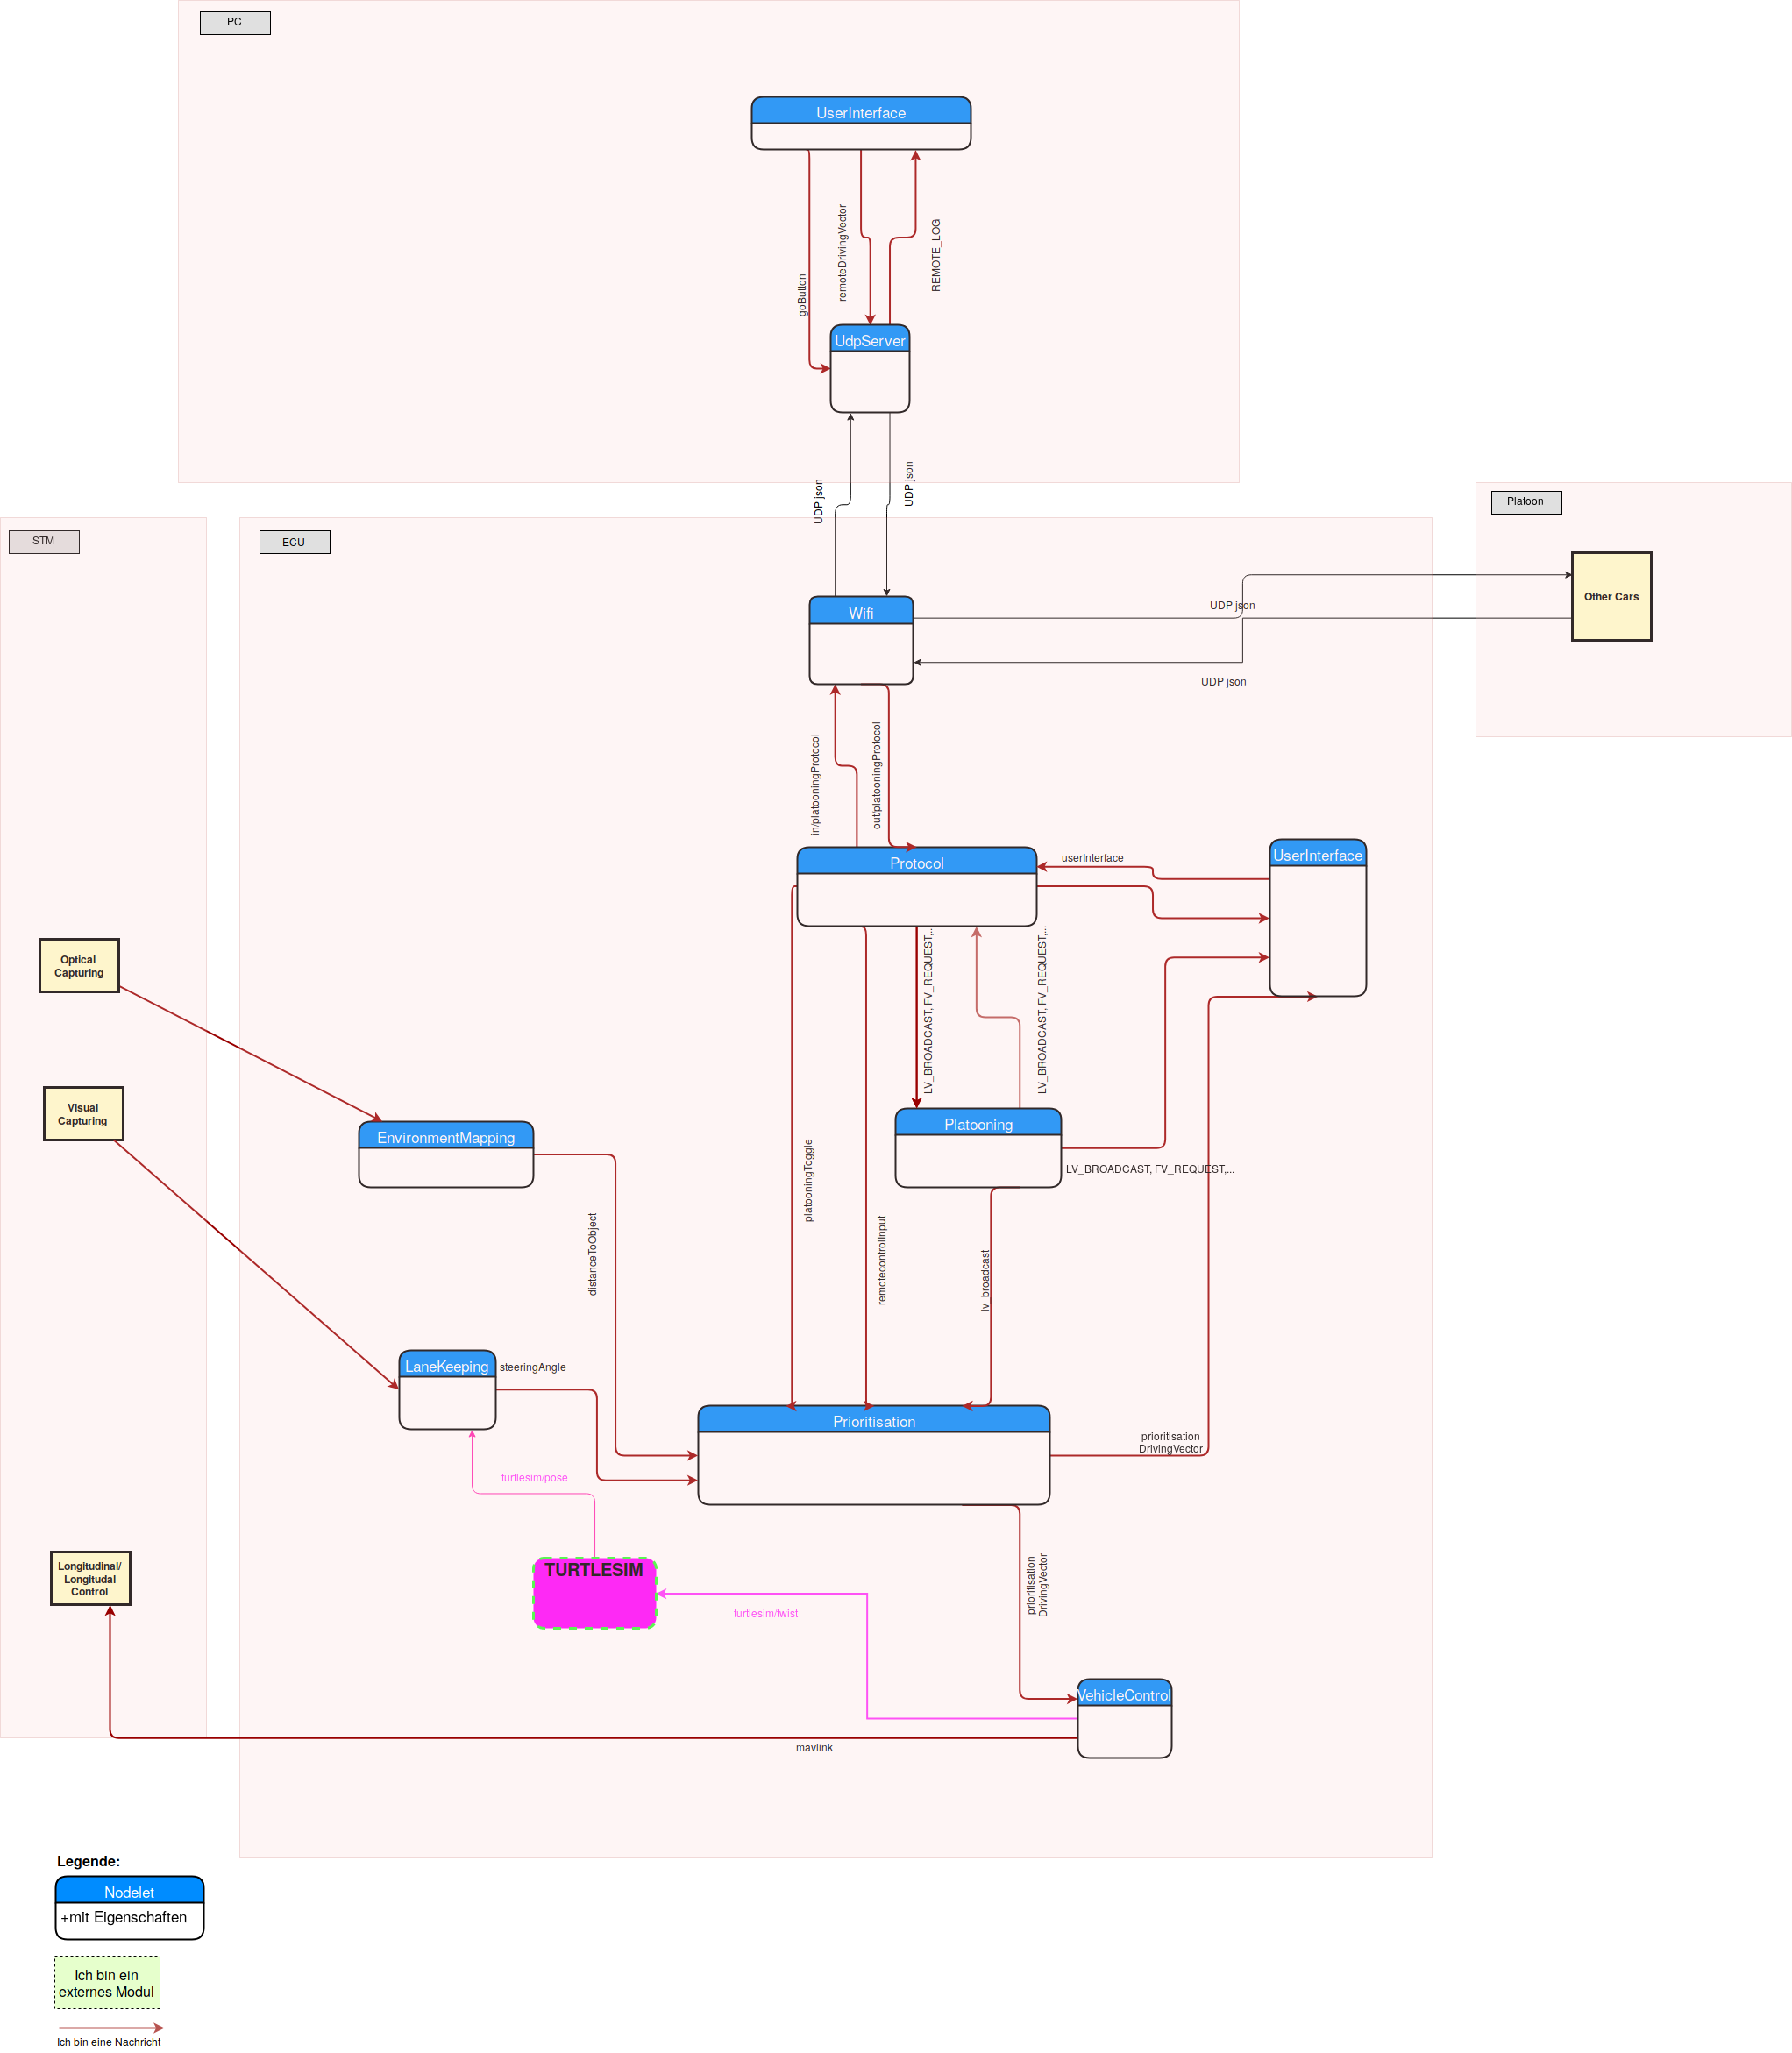
\includegraphics[width=\textwidth]{platooning_architecture.png}

		\subsection{ROS}
		\label{ros}
		ROS, kurz für robot operating system, ist entgegen des Namens ein Framework, welches Werkzeuge zur Entwicklung von Software für Roboter bereitstellt. Dazu gehört ein System wie Module bzw. Nodelets miteinander kommunizieren können, Visualisierer der Interaktion der Nodelets und Simulatoranbindungen.\\

		Die wichtigsten Komponenten von ROS sind die ROS Nodelets, Topics und Messages. \\

		Die Nodelets sind die einzelnen Softwarekomponenten. Sie werden durch einen Nodeletmanager geladen und initiiert. Die Interaktion der Nodelets erfolgt meist über Topics auf denen Messages versandt werden. Der Nodeletmanager bzw. der ROS Master registriert welche Nodelets auf einer Topic Nachrichten verschicken und welche Nodelets informiert werden müssen, wenn auf einer Topic eine neue Nachricht versandt wurde.\\

		Einen tieferen Einblick findet man unter\\
		https://www.generationrobots.com/blog/de/2016/03/ros-robot-operating-system/

		\subsection{Coding-Standard}
		\label{coding_standard}
			Die im Projekt verwendete Programmiersprache ist C++, da diese mit dem ROS-Betriebssystem kompatibel ist.
			Um die Verständlichkeit und Lesbarkeit innerhalb der Projektgruppe zu gewährleisten, haben wir uns auf
			bestimmte syntaktische Standards geeinigt. Eine erste Orientierung boten der Google C++ Style Guide\cite{googleTest} und die C++ Core Guidelines\cite{cppCoreGuide}.

			Der Code ist aufgeteilt in Deklarations- und Definitionsteil, sprich: in Header- und CPP-Dateien.
			Klassennamen werden mit großem Anfangsbuchstaben geschrieben, Variablen mit kleinen. Klassenvariablen enden zudem
			auf einem Unterstrich. Zur besseren Lesbarkeit werden die Namen im sog. \emph{snake case}\footnote{Die einzelnen
			Worte des Kompositums werden durch Unterstriche getrennt, z.B.: important\_value} geschrieben.
			Die Einrückung mittels Tabulator beträgt vier Leerzeichen.

			Die von uns verwendete IDE, vgl. dazu Kapitel \ref{umfeld}, bot die Möglichkeit, den Google C++ Style Guide und andere Code-Konventionen zu unterstützen.

		\subsection{Modulbeschreibung}
		\label{modulbeschreibung}
		% Beschreibung der Nodes inkl. (Aktivitäts-)Diagramme
			\subsubsection{Prioritization}
			\label{prioritization}
				\paragraph{Aufgabe} Das Prioritization-Nodelet erhält Fahrdaten vom Platooning-Nodelet und der MessageDistribution und entscheidet dann, wie sich das Fahrzeug zu verhalten hat. Er entscheidet also zwischen verschiedenen Steuersignalen, welches gerade benutzt werden soll.
				\paragraph{Assoziationen} Das Prioritization-Nodelet ist Subscriber vom Platooning-Nodelet und dem MessageDistribution-Nodelet. Es ist Publisher für den LongitudinalProcessing-Nodelet und das LateralProcessing-Nodelet.
				\paragraph{Attribute}
					\begin{itemize}
						\item float \_speed\_ Die Geschwindigkeit, mit der das Auto fahren soll.
						\item float \_distance\_ Die Distanz, die innerhalb des Platoons zwischen den Fahrzeugen beibehalten werden soll.
						\item float target\_angle\_ Der Winkel, auf den die Steuerung eingestellt werden soll.
						\item PrioritizationState state\_ Gibt an, in welchem Modus das Prioritization-Nodelet derzeit ist. Der Modus gibt an, ob das Auto derzeit zum Beispiel die Fernsteuerung oder die Nachrichten aus dem Platoon priorisieren soll.
					\end{itemize}
				\paragraph{Methoden}
					\subparagraph{hndl\_remotecontrolInput} Wird aufgerufen, wenn Daten der RemoteControl empfangen wurden und veröffentlicht diese via Topic, falls das Auto im State REMOTECONTROL ist.
					\subparagraph{hndl\_platooningToggle} Wird aufgerufen, wenn eine PlatooningToggleMessage empfangen wird. Setzt die Variable state\_ dann entsprechend auf PLATOONING.
					\subparagraph{hndl\_platooningState} Wird aufgerufen, sobald eine PlatooningState Message empfangen wurde. Wenn state\_ auf Platooning gesetzt ist, sorgt die Methode dafür, dass das Auto als FV zur Kolonne aufschließt. ‘
				\paragraph{Input}
				    \begin{itemize}
				        \item remotecontrolInput von Nodelet MessageDistribution
				        \item remotecontrolToggle von Nodelet MessageDistribution
				        \item platooningToggle von Nodelet MessageDistribution
				        \item platooningState von Nodelet Platooning
				    \end{itemize}
				\paragraph{Output}
				    \begin{itemize}
				        \item targetSpeed an Nodelet LongitudinalProcessing
				        \item targetDistance an Nodelet LongitudinalProcessing
				        \item targetAngle an Nodelet LateralProcessing
				    \end{itemize}

			\subsubsection{Platooning}
			\label{platooning}
				\paragraph{Aufgabe} Das Platooning-Nodelet kommuniziert mit den anderen Fahrzeugen und tauscht mit diesen Daten aus. Zu den Daten gehören Geschwindigkeit des Platoons, die im Platoon einzuhaltende Distanz, Heartbeats sowie Broadcasts.
				\paragraph{Assoziationen} Zu den Subscribern des Platooning-Nodelet gehören das Prioritization-Nodelet und das MessageDistribution-Nodelet. Publisher für das Platooning-Nodelet ist das MessageDistribution-Nodelet.
				\paragraph{Methoden}
					\subparagraph{}
				\paragraph{Input}
				    \begin{itemize}
    					\item platooningToggle von Nodelet MessageDistribution
    					\item in/FV\_REQUEST von Nodelet MessageDistribution
    					\item in/LV\_BROADCAST von Nodelet MessageDistribution
    				\end{itemize}
				\paragraph{Output}
					\begin{itemize}
    					\item PlatooningState an Nodelet Prioritization
    					\item out/FV\_REQUEST an Nodelet MessageDistribution
    					\item out/LV\_BROADCAST an Nodelet MessageDistribution
    				\end{itemize}

		    \subsubsection{User Interface}
			\label{user_interfcae}
				\paragraph{Aufgabe} Das UserInterface-Nodelet zeigt dem Nutzer aktuelle Daten des Fahrzeugs an. Dazu gehören zum Beispiel Nachrichten aus dem Platoon, Geschwindigkeit und Distanz zu anderen Objekten. Aus diesen Daten soll der Nutzer das Verhalten des Autos nachvollziehen können.
				\paragraph{Assoziationen} Das UserInterface-Nodelet ist Subscriber vom UdpServer-Nodelet.
				\paragraph{Attribute}
					\begin{itemize}
					    \item Alle Attribute sind selbsterkl"arend
					\end{itemize}
				\paragraph{Methoden}
					\subparagraph{hndl\_*} (Wobei * eine der verschiedenen Variablen oder Nachrichten ist.) Für jede Variable (wie zum Beispiel Geschwindigkeit, Beschleunigung etc.) gibt es im UserInterface-Nodelet eine Methode. Die Methoden empfangen die jeweilige Variable und geben diese dann auf dem User Interface aus.
				\paragraph{Input}
				    \begin{itemize}
				        \item userInterfaceData von Nodelet UdpServer
				    \end{itemize}
				\paragraph{Output}
				    \begin{itemize}
				        \item remoteControlInput an Nodelet UdpServer
				        \item platooningToggle an Nodelet UdpServer
				        \item remoteControlToggle an Nodelet UdpServer
				    \end{itemize}

			\subsubsection{Message Translation}
			\label{message_translation}
				\paragraph{Aufgabe} Der MessageDistribution-Node ist dafür verantwortlich, Messages in Datentypen zu übersetzen, damit diese dann von den unterschiedlichen Nodes verwendet werden können.
				\paragraph{Assoziationen} Der MessageDistribution-Node ist Subscriber vom RadioInterface-Node und dem Platooning-Node. Er ist Publisher für den UserInterface-Node, den RadioInterface-Node, den Platooning-Node und den Prioritization-Node.
				\paragraph{Attribute}
					\subparagraph{Tolles Attribut A}
				\paragraph{Methoden}
					\subparagraph{Tolle Methode A}
				\paragraph{Input}
				\paragraph{Output}

			\subsubsection{Message Distribution}
			\label{message_distribution}
				\paragraph{Aufgabe} Das MessageDistribution-Nodelet erhält alle eingehenden Nachrichten. Je nach Typ werden diese Nachrichten dann vom MessageDistribution-Nodelet auf den passenden Topics veröffentlicht. Dadurch erhalten alle Nodelet immer die richtigen Nachrichten.
				\paragraph{Assoziationen} ???
				\paragraph{Attribute}
				    \begin{itemize}
				        \item Alle Attribute sind selbsterklärend.
				    \end{itemize}
				\paragraph{Methoden}
                    \subparagraph{hndl\_platooningIn} Erkennt, welche Art von Message empfangen wurde, dekodiert diese und veröffentlicht sie auf dem entsprechenden Topic.
					\subparagraph{hndl\_lv\_broadcast} Verpackt die zu übertragenden Daten in eine LV\_BROADCAST-Nachricht und veröffentlicht diese an das Platoon.
					\subparagraph{hndl\_lv\_accept} Verpackt die zu übertragenden Daten in eine LV\_ACCEPT-Nachricht und veröffentlicht diese an das Platoon.
					\subparagraph{hndl\_lv\_reject} Verpackt die zu übertragenden Daten in eine LV\_REJECT-Nachricht und veröffentlicht diese an das Platoon.
                	\subparagraph{hndl\_fv\_heartbeat} Verpackt die zu übertragenden Daten in eine FV\_HEARTBEAT-Nachricht und veröffentlicht diese an das Platoon.
                    \subparagraph{hndl\_fv\_leave} Verpackt die zu übertragenden Daten in eine FV\_LEAVE-Nachricht und veröffentlicht diese an das Platoon.
                	\subparagraph{hndl\_fv\_request} Verpackt die zu übertragenden Daten in eine FV\_REQEUEST-Nachricht und veröffentlicht diese an das Platoon.
                	\subparagraph{hndl\_ui} Verpackt die zu übertragenden Daten in eine REMOTE\_USERINTERFACE-Nachricht und veröffentlicht diese im Netzwerk.
				\paragraph{Input} ???
				\paragraph{Output} ???

			\subsubsection{MessageTypes}
			\label{messages_types}
				\paragraph{Aufgabe} ??
				\paragraph{Assoziationen}
				\paragraph{Attribute}
					\subparagraph{Tolles Attribut A}
				\paragraph{Methoden}

				\paragraph{Input}
				\paragraph{Output}

			\subsubsection{Distance Processing}
			\label{distance_processing}
				\paragraph{Aufgabe} Der DistanceProcessing-Nodelet misst, wie weit er von den nächstgelegenen Objekten entfernt ist und stellt diese Information anderen Knoten zur Verfügung.
				\paragraph{Assoziationen} Der DistanceProcessing-Nodelet erhält seine Informationen von einem Ultraschall-Sensor. Es ist Publisher für das LongitudinalProcessing-Nodelet.
				\paragraph{Attribute}
					\subparagraph{Tolles Attribut A}
				\paragraph{Methoden}
					\subparagraph{Tolle Methode A}
				\paragraph{Input}
				\paragraph{Output}

			\subsubsection{Longitudinal Processing}
			\label{longitudinal_processing}
				\paragraph{Aufgabe} Das LongitudinalProcessing-Nodelet ist für die Beschleunigung des Autos verantwortlich. Er erhält die gewünschte Geschwindigkeit aus dem Prioritization-Nodelet und schickt dann die gewünschte Beschleunigung an den VehicleControl-Nodelet.
				\paragraph{Assoziationen} Der LongitudinalProcessing-Nodelet ist Subscriber vom Prioritization-Nodelet, dem DistancePreprocessing-Nodelet und dem Speed Sensor. Es ist Publisher für das VehicleControl-Nodelet.
				\paragraph{Attribute}
					\subparagraph{Tolles Attribut A}
				\paragraph{Methoden}
					\subparagraph{hndl\_distance\_from\_sensor} Empfängt den Abstand vom Sensor *TODO* (Was für ein Sensor?) und prüft ob es zwei Messungen gibt (warum das?). Ist das der Fall so wird die Beschleunigung angepasst und die ensprechenden Flags für die erfolgte Distanzmessung gesetzt.

					\subparagraph{hndl\_target\_distance} Empfängt die aktuelle Zieldistanz *TODO* (platoon distance?) und prüft ob diese in einem angemessenen Bereich liegt. Ist das der Fall so wird die Zieldistanz des der PD Steuerung übermittelt. Bei unangemessen niedriger Zieldistanz (kleiner als 0,5) wird diese auf 1 gesetzt.

					\subparagraph{hndl\_current\_velocity} Empfängt die aktuellen Beschleunigungsdaten. Falls diese von der derzeitigen Beschleunigung abweicht, wird der Wert angepasst und das entsprechende Flag gesetzt.

					\subparagraph{hndl\_targetSpeed} Empfängt die aktuelle Zielgeschwindigkeit. Falls diese von der derzeitigen Geschwindigkeit abweicht, wird der Wert angepasst und das entsprechende Flag gesetzt.

					\subparagraph{update\_velocity} Berechnet die Beschleunigung anhand der aktuellen Zielgeschwindigkeit, Zieldistanz, Beschleunigung und des Abstands. Außerdem wird die relative Geschwindigkeit anhand der Veränderung des Abstands berechnet um daraus die Anpassung des Zielabstands zu berechnen und die Beschleunigung zu versenden.

					\subparagraph{check\_dead\_datasrc} Verarbeitet eine Ablaufzeit, in der auf eine Aktualisierung des Abstands- und Beschleunigungsmessung gewartet wird. Läuft die Zeit ab, wird derzeit ein Notstopp durchgeführt.

					\subparagraph{calulate\_velocity} Hilfsfunktion zur Berechnung der aktuellen Beschleunigung.

					\subparagraph{set\_target\_position} Hilfsfunktion zum Berechnen und Setzen der Zielposition.


				\paragraph{Input}
				    \begin{itemize}
				    	\item in/platooningProtocol von Node MessageDistribution
				    	\item Daten vom UdpServer
				    \end{itemize}

				\paragraph{Output}

			\subsubsection{Radio Interface}
			\label{radio_interface}
				\paragraph{Aufgabe} Das RadioInterface-Nodelet wickelt den Nachrichtenverkehr über UDP ab. Er benutzt den UDP-Server, um das Senden und Empfangen von Netzwerk-Nachrichten über UDP zu ermöglichen.
				\paragraph{Assoziationen} Das RadioInterface-Nodelet ist
				\paragraph{Attribute}
					\begin{itemize}
					    \item std::unique\_ptr<UdpServer> platooning\_server\_ptr\_ Ein einmaliger Pointer für den Platooning Server.
					    \item std::unique\_ptr<UdpServer> controller\_server\_ptr\_ Ein einmaliger Pointer für den Controller Server.
					\end{itemize}
				\paragraph{Methoden}
				    \subparagraph{hndl\_platoonProtocolOut} Sendet Nachrichten in das Netzwerk. Je nach MessageType muss die Nachricht anders verschickt werden. Daher wird hierfür eine extra Methode benötigt.
					\subparagraph{hndl\_radio\_receive} Kümmert sich um die empfangenen Nachrichten aus dem Netzwerk. Je nach MessageType muss mit den empfangenen Nachrichten anders verfahren werden.
				\paragraph{Input}
				    \begin{itemize}
				        \item in/platooningProtocol von Nodelet MessageDistribution
				        \item Daten vom UdpServer
				    \end{itemize}
				\paragraph{Output}
				    \begin{itemize}
				        \item out/platooningProtocol an Nodelet MessageDistribution
				        \item Daten an UdpServer
				    \end{itemize}

		    \subsubsection{UdpServer}
			\label{udpserver}
				\paragraph{Aufgabe} Das UdpServer-Nodelet wird vom RadioInterface-Nodelet verwendet, um den Nachrichtenverkehr über das Netzwerk realisieren zu können.
				\paragraph{Assoziationen} Das UdpServer-Nodelet ist Subscriber vom UserInterface-Nodelet und Publisher für den UserInterface-Nodelet.
				\paragraph{Attribute}
					\subparagraph{Tolles Attribut A}
				\paragraph{Methoden}
					\subparagraph{Tolle Methode A}
				\paragraph{Input}
				\paragraph{Output}

	\section{Tests}
	\label{tests}
		\subsection{Test-Standard}
		\label{test_standard}
		Als Testing Framework für unsere Unit Tests wurde im Rahmen des Projektes zuerst Google Test verwendet.
		Hierbei handelt es sich um eine plattformübergreifende\footnote{Verfügbar auf den Betriebssystemen Linux, Windows, Mac OS},
		von Google entwickelte Test-Bibliothek für die Programmiersprache C++. Diese zeichnet sich durch schnelle Performanz und
		Wiederverwertbarkeit aus. Letzteres war im Projekt von Vorteil, da die gleichen Tests auf unterschiedlichen Systemen der
		Projektteilnehmer liefen, ohne Modifizierungen vornehmen zu müssen. Des Weiteren ist es mit Google Test möglich, die Test
		isoliert voneinander ablaufen zu lassen, um im Falle eines gescheiterten Test die Fehlerquelle gezielter zu finden. Die von unserer Gruppe weitestgehend verwendete IDE, vgl. dazu Abschnitt \ref{umfeld}, unterstützt zudem die Integration von Google Test.

		Einander ähnelnde Test bzw. Tests, die sich auf eine bestimmte Komponente beziehen, können in sog. \emph{Test Cases}
		organisiert und bei Bedarf einzeln oder im Verbund getestet werden. In diesem Zusammenhang muss jedoch erwähnt werden,
		dass der Ausdruck \emph{Test Case} dem ISTQB\footnote{International Software Testing Qualificatios Board}-Ausdruck
		\emph{Test Suite} entspricht \cite{google}.

		Die Testergebnisse werden automatisch generiert und in der Konsole ausgegeben. Bei Bedarf kann ein XML-Report erzeugt werden.

		Eine beispielhafte Anleitung zum globalen Einbinden von Google Test für das Betriebssystem Ubuntu 16.04 befindet sich im Anhang \ref{appendix:gtest_install}.

		Im späteren Verlauf stellte sich die Integration von Google Test mit ROS als schwierig heraus: Die meisten Tests benötigen einen laufenden ROS master, welcher entweder aus per launch-Datei gestartet werden muss oder manuell selbst. Dies erschwert das gewünschte automatisierte Testprotokoll.	Deswegen wurde ein einfaches eigenes Framework aufgesetzt. Siehe dazu die Doku zu den Modulen Modultest und Integrationstest.

		Alternativ ist eine Integration von Google Test mit ROS Test möglich, wurde im Projekt aufgrund des weiteren Aufwands jedoch abgelehnt.

		% Probleme in Verbindung mit ROS, Erzeugen von Reports zB als xml output

		\subsection{Test-Cases}
		\label{test_cases}
			\subsubsection{Nodelet Prioritization}
			\label{node_prioritization}
				\paragraph{Test 1:}{Test Geschwindigkeitskontrolle durch Remote Control}
				\paragraph{Beschreibung:} Getestet wird, ob Prioritization Nodelet auf Geschwindigkeitskontrolle durch Remote Control reagiert.
				\paragraph{Input:}
				\begin{itemize} \itemsep-0.5em
					\item \textbf{Vehicle ID:} \emph{vehicle\_id = 1}
					\item \textbf{Vorgegebene Geschwindigkeit:} \emph{remote\_speed = 2}
					\item \textbf{Vorgegebener Steuerungswinkel:} \emph{remote\_angle = 3}
				\end{itemize}
				\paragraph{Erwarteter Output:}
				\begin{itemize} \itemsep-0.5em
					\item \textbf{Geschwindigkeit:} \emph{velocity = 2}
					\item \textbf{Steuerungswinkel:} \emph{steering\_angle = 3}
				\end{itemize}
				\paragraph{Test 2:}{Test Remote Control Toggle}
				\paragraph{Beschreibung:} Es wird überprüft, ob das Abschalten der Remote Control funktioniert.
				\paragraph{Input:}
				\begin{itemize} \itemsep-0.5em
					\item \textbf{Remote Control:} \emph{enable\_remotecontrol = false}
					\item \textbf{Vehicle ID:} \emph{vehicle\_id = 1}
					\item \textbf{Vorgegebene Geschwindigkeit:} \emph{remote\_speed = 2}
					\item \textbf{Vorgegebener Steuerungswinkel:} \emph{remote\_angle = 3}
				\end{itemize}
				\paragraph{Erwarteter Output:}
				\begin{itemize} \itemsep-0.5em
					\item \textbf{Empfang von Daten:} \emph{vehiclecontrol\_received = false}
				\end{itemize}

				\paragraph{Test 3:} {Test Geschwindigkeitskontrolle durch Platooning}
				\paragraph{Beschreibung:} Getestet wird, ob das Prioritization Nodelet auf Geschwindigkeitsvorgabe von Platooning reagiert.
				\paragraph{Input:}
				\begin{itemize} \itemsep-0.5em
					\item \textbf{Vehicle ID:} \emph{vehicle\_id = 1}
					\item \textbf{Leader Vehicle:} \emph{i\_am\_LV = false}
					\item \textbf{Follower Vehicle:} \emph{i\_am\_FV = true}
					\item \textbf{Inner Platoon Distance:} \emph{ipd = 1}
					\item \textbf{Platoon Speed:} \emph{ps = 1}
					\item \textbf{Platoon ID:} \emph{platoon\_id = 1}
					\item \textbf{Platooning State:} \emph{platooning\_state = RUNNING}
					\item \textbf{Platoon Members:} \emph{platoon\_members = \{ 1, 2 \}}
				\end{itemize}
				\paragraph{Erwarteter Output:}
				\begin{itemize} \itemsep-0.5em
					\item \textbf{Geschwindigkeit:} \emph{velocity = 1.0f}
					\item \textbf{Steuerungswinkel:} \emph{steering\_angle = 0.0f}
				\end{itemize}

				\paragraph{Test 4:} {Test Platooning Toggle}
				\paragraph{Beschreibung:} Es wird überprüft, ob das Abschalten der Kontrolle durch das Platooning Nodelet funktioniert.
				\paragraph{Input:}
				\begin{itemize} \itemsep-0.5em
					\item \textbf{Platooning:} \emph{enable\_platooning = false}
					\item \textbf{Vehicle ID:} \emph{vehicle\_id = 1}
				\end{itemize}
				\paragraph{Erwarteter Output:}
				\begin{itemize} \itemsep-0.5em
					\item \textbf{Empfang von Daten:} \emph{vehiclecontrol\_received = false}
				\end{itemize}

			\subsubsection{Nodelet Longitudinal Processing}
			\label{node_longitudinal_processing}
			\paragraph{Test 1:}{Test Geschwindigkeitsupdate}
			\paragraph{Beschreibung:} Getestet wird, ob Geschwindigkeitsanpassung durch das Longitudinal Processing Nodelet funktioniert.
			\paragraph{Input:}
			\begin{itemize} \itemsep-0.5em
				\item \textbf{Ziel Geschwindigkeit:} \emph{target\_speed = 3}
				\item \textbf{Ziel Distanz:} \emph{distance = 3}
				\item \textbf{Aktuelle Geschwindigkeit:} \emph{current\_speed = 3}
			\end{itemize}
			\paragraph{Erwarteter Output:}
			\begin{itemize} \itemsep-0.5em
				\item \textbf{Geschwindigkeit:} \emph{speed = 3}
			\end{itemize}
			\paragraph{Test 2:}{Test Geschwindigkeitsanpassung zu LV}
			\paragraph{Beschreibung:} Es wird überprüft, ob FV auf beschleunigendes LV reagiert.
			\paragraph{Input:}
			\begin{itemize} \itemsep-0.5em
				\item \textbf{Ziel Geschwindigkeit:} \emph{target\_speed = 8}
				\item \textbf{Ziel Distanz:} \emph{distance = 1}
				\item \textbf{Aktuelle Geschwindigkeit:} \emph{current\_speed = 2}
			\end{itemize}
			\paragraph{Erwarteter Output:}
			\begin{itemize} \itemsep-0.5em
				\item \textbf{Distanz:} \emph{(lv\_pos - fv\_pos \textgreater 0) \&\& (lv\_pos - fv\_pos \textless 1)}
			\end{itemize}

			\subsubsection{Nodelet Platooning}
			\label{node_platooning}
			\paragraph{Test 1:}{Test Platoon Erstellung}
			\paragraph{Beschreibung:} Es wird überprüft, ob die Platoon-Einstellungen übernommen werden.
			\paragraph{Input:}
			\begin{itemize} \itemsep-0.5em
				\item \textbf{Platooning Toogle:} \emph{enable\_platooning = true}
				\item \textbf{Platoon Geschwindigkeit:} \emph{platoon\_speed = 3}
				\item \textbf{Innerer Platoon Abstand:} \emph{inner\_platoon\_distance = 4}
			\end{itemize}
			\paragraph{Erwarteter Output:}
			\begin{itemize} \itemsep-0.5em
				\item \textbf{Platoon Mitglieder:} \emph{platoon\_members.empty() = false}
				\item \textbf{Innerer Platoon Abstand:} \emph{inner\_platoon\_distance = 4}
				\item \textbf{Platoon Geschwindigkeit:} \emph{platoon\_speed = 3}
				\item \textbf{Platoon Zustand:} \emph{platooning\_state = CREATING}
			\end{itemize}

			\paragraph{Test 2:}{Test FV Anfrage an LV}
			\paragraph{Beschreibung:} Es wird überprüft, ob FV Request gelingt.
			\paragraph{Input:}
			\begin{itemize} \itemsep-0.5em
				\item \textbf{Vehicle, das Request sendet:} \emph{src\_vehicle = 5}
			\end{itemize}
			\paragraph{Erwarteter Output:}
			\begin{itemize} \itemsep-0.5em
				\item \textbf{Vehicle, von dem Request kommt:} \emph{dst\_vehicle = 5}
			\end{itemize}

			\subsubsection{Nodelet MessageDistribution}
			\label{node_message_distribution}
			\paragraph{Test 1:}{Test LV Broadcast 1
			\paragraph{Beschreibung:} Test LV Broadcast von IN\_PLATOONING\_MSG zu IN\_LV\_BROADCAST.
			\paragraph{Input:}
			\begin{itemize} \itemsep-0.5em
				\item \textbf{Message Type:} \emph{message\_type = IN\_PLATOONING\_MSG}
				\item \textbf{vehicle id:} \emph{src\_vehicle = 3}
			\end{itemize}
			\paragraph{Erwarteter Output:}
			\begin{itemize} \itemsep-0.5em
				\item \textbf{Vehicle, von dem LV Broadcast kommt:} \emph{src\_vehicle = 3}
				\item \textbf{Message Type:} \emph{message\_type = IN\_LV\_BROADCAST}
			\end{itemize}

			\paragraph{Test 2:}{Test LV Broadcast 2}
			\paragraph{Beschreibung:} Test LV Broadcast von OUT\_LV\_BROADCAST zu OUT\_PLATOONING\_MSG.
			\paragraph{Input:}
			\begin{itemize} \itemsep-0.5em
				\item \textbf{Message Type:} \emph{message\_type = OUT\_PLATOONING\_MSG}
			\end{itemize}
			\paragraph{Erwarteter Output:}
			\begin{itemize} \itemsep-0.5em
				\item \textbf{Message Type:} \emph{message\_type = LV\_BROADCAST}
			\end{itemize}

			\paragraph{Test 3:}{Test LV Accept Msg}
			\paragraph{Beschreibung:} Test ob LV Accept Msg funktioniert.
			\paragraph{Input:}
			\begin{itemize} \itemsep-0.5em
				\item \textbf{Message Type:} \emph{message\_type = IN\_PLATOONING\_MSG}
				\item \textbf{Source Vehicle:} \emph{src\_vehicle = 3}
				\item \textbf{Platoon ID:} \emph{platoon\_id = 4}
				\item \textbf{Destination Vehicle:} \emph{dst\_vehicle = 5}
			\end{itemize}
			\paragraph{Erwarteter Output:}
			\begin{itemize} \itemsep-0.5em
				\item \textbf{Message Type:} \emph{message\_type = LV\_ACCEPT}
				\item \textbf{Source Vehicle:} \emph{src\_vehicle = 3}
				\item \textbf{Platoon ID:} \emph{platoon\_id = 4}
				\item \textbf{Destination Vehicle:} \emph{dst\_vehicle = 5}
			\end{itemize}

			\paragraph{Test 4:}{Test LV\_Accept zu OUT\_PLATOONING\_MSG}
			\paragraph{Beschreibung:} Test Msg LV Accept zu Out Platooning.
			\paragraph{Input:}
			\begin{itemize} \itemsep-0.5em
				\item \textbf{Message Type:} \emph{message\_type = LV\_Accept}

			\end{itemize}
			\paragraph{Erwarteter Output:}
			\begin{itemize} \itemsep-0.5em
				\item \textbf{Message Type:} \emph{message\_type = OUT\_PLATOONING\_MSG}
			\end{itemize}

			\paragraph{Test 5:}{Test IN\_PLATOONING\_MSG zu IN\_LV\_REJECT}
			\paragraph{Beschreibung:} Test Msg In Platooning zu LV Reject.
			\paragraph{Input:}
			\begin{itemize} \itemsep-0.5em
				\item \textbf{Message Type:} \emph{message\_type = IN\_PLATOONING\_MSG}
				\item \textbf{vehicle id:} \emph{src\_vehicle = 3}
			\end{itemize}
			\paragraph{Erwarteter Output:}
			\begin{itemize} \itemsep-0.5em
				\item \textbf{Message Type:} \emph{message\_type = IN\_LV\_REJECT}
				\item \textbf{vehicle id:} \emph{src\_vehicle = 3}
			\end{itemize}

			\paragraph{Test 6:}{Test IN\_PLATOONING\_MSG zu IN\_FV\_HEARTBEAT}
			\paragraph{Beschreibung:} Test Msg In Platooning zu FV Heartbeat.
			\paragraph{Input:}
			\begin{itemize} \itemsep-0.5em
				\item \textbf{Message Type:} \emph{message\_type = IN\_PLATOONING\_MSG}
				\item \textbf{vehicle id:} \emph{src\_vehicle = 3}
			\end{itemize}
			\paragraph{Erwarteter Output:}
			\begin{itemize} \itemsep-0.5em
				\item \textbf{Message Type:} \emph{message\_type = IN\_FV\_HEARTBEAT}
				\item \textbf{vehicle id:} \emph{src\_vehicle = 3}
			\end{itemize}

			\paragraph{Test 7:}{Test OUT\_FV\_HEARTBEAT zu OUT\_PLATOONING\_MSG}
			\paragraph{Beschreibung:} Test Msg FV Heartbeat zu Platooning.
			\paragraph{Input:}
			\begin{itemize} \itemsep-0.5em
				\item \textbf{Message Type:} \emph{message\_type = OUT\_FV\_HEARTBEAT}
			\end{itemize}
			\paragraph{Erwarteter Output:}
			\begin{itemize} \itemsep-0.5em
				\item \textbf{Message Type:} \emph{message\_type = OUT\_PLATOONING\_MSG}
			\end{itemize}

			\paragraph{Test 8:}{Test IN\_PLATOONING\_MSG zu IN\_FV\_LEAVE}
			\paragraph{Beschreibung:} Test Msg In Platooning zu FV Leave.
			\paragraph{Input:}
			\begin{itemize} \itemsep-0.5em
				\item \textbf{Message Type:} \emph{message\_type = IN\_PLATOONING\_MSG}
				\item \textbf{vehicle id:} \emph{src\_vehicle = 3}
			\end{itemize}
			\paragraph{Erwarteter Output:}
			\begin{itemize} \itemsep-0.5em
				\item \textbf{Message Type:} \emph{message\_type = IN\_FV\_LEAVE}
				\item \textbf{vehicle id:} \emph{src\_vehicle = 3}
			\end{itemize}

			\paragraph{Test 9:}{Test OUT\_FV\_LEAVE zu OUT\_PLATOONING\_MSG}
			\paragraph{Beschreibung:} Test Msg In FV Leave zu Platooning.
			\paragraph{Input:}
			\begin{itemize} \itemsep-0.5em
				\item \textbf{Message Type:} \emph{message\_type = OUT\_FV\_LEAVE}
			\end{itemize}
			\paragraph{Erwarteter Output:}
			\begin{itemize} \itemsep-0.5em
				\item \textbf{Message Type:} \emph{message\_type = OUT\_PLATOONING\_MSG}
			\end{itemize}

			\paragraph{Test 10:}{Test IN\_PLATOONING\_MSG zu IN\_FV\_REQUEST}
			\paragraph{Beschreibung:} Test Msg In Platooning zu FV request.
			\paragraph{Input:}
			\begin{itemize} \itemsep-0.5em
				\item \textbf{Message Type:} \emph{message\_type = IN\_PLATOONING\_MSG}
				\item \textbf{vehicle id:} \emph{src\_vehicle = 3}
			\end{itemize}
			\paragraph{Erwarteter Output:}
			\begin{itemize} \itemsep-0.5em
				\item \textbf{Message Type:} \emph{message\_type = IN\_FV\_REQUEST}
				\item \textbf{vehicle id:} \emph{src\_vehicle = 3}
			\end{itemize}

			\paragraph{Test 11:}{Test OUT\_FV\_REQUEST zu OUT\_PLATOONING\_MSG}
			\paragraph{Beschreibung:} Test Msg Out FV request zu Out Platooning.
			\paragraph{Input:}
			\begin{itemize} \itemsep-0.5em
				\item \textbf{Message Type:} \emph{message\_type = OUT\_FV\_REQUEST}
			\end{itemize}
			\paragraph{Erwarteter Output:}
			\begin{itemize} \itemsep-0.5em
				\item \textbf{Message Type:} \emph{message\_type = OUT\_PLATOONING\_MSG}
			\end{itemize}

			\paragraph{Test 12:}{Test IN\_PLATOONING\_MSG zu INPUT\_REMOTECONTROL}
			\paragraph{Beschreibung:} Test Msg In Platooning zu Input Remote control request.
			\paragraph{Input:}
			\begin{itemize} \itemsep-0.5em
				\item \textbf{Message Type:} \emph{message\_type = IN\_PLATOONING\_MSG}
				\item \textbf{vehicle id:} \emph{src\_vehicle = 3}
			\end{itemize}
			\paragraph{Erwarteter Output:}
			\begin{itemize} \itemsep-0.5em
				\item \textbf{Message Type:} \emph{message\_type = INPUT\_REMOTECONTROL}
				\item \textbf{vehicle id:} \emph{src\_vehicle = 3}
			\end{itemize}

			\paragraph{Test 13:}{Test IN\_PLATOONING\_MSG zu TOGGLE\_REMOTECONTROL}
			\paragraph{Beschreibung:} Test Msg In Platooning zu Remote control toggle.
			\paragraph{Input:}
			\begin{itemize} \itemsep-0.5em
				\item \textbf{Message Type:} \emph{message\_type = IN\_PLATOONING\_MSG}
				\item \textbf{vehicle id:} \emph{src\_vehicle = 3}
			\end{itemize}
			\paragraph{Erwarteter Output:}
			\begin{itemize} \itemsep-0.5em
				\item \textbf{Message Type:} \emph{message\_type = TOGGLE\_REMOTECONTROL}
				\item \textbf{vehicle id:} \emph{src\_vehicle = 3}
			\end{itemize}

			\paragraph{Test 14:}{Test IN\_PLATOONING\_MSG zu TOGGLE\_PLATOONING}
			\paragraph{Beschreibung:} Test Msg In Platooning zu platooning toggle.
			\paragraph{Input:}
			\begin{itemize} \itemsep-0.5em
				\item \textbf{Message Type:} \emph{message\_type = IN\_PLATOONING\_MSG}
				\item \textbf{vehicle id:} \emph{src\_vehicle = 3}
			\end{itemize}
			\paragraph{Erwarteter Output:}
			\begin{itemize} \itemsep-0.5em
				\item \textbf{Message Type:} \emph{message\_type = TOGGLE\_PLATOONING}
				\item \textbf{vehicle id:} \emph{src\_vehicle = 3}
			\end{itemize}

			\paragraph{Test 15:}{Test IN\_PLATOONING\_MSG zu USERINTERFACE}
			\paragraph{Beschreibung:} Test Msg In Platooning zu user interface.
			\paragraph{Input:}
			\begin{itemize} \itemsep-0.5em
				\item \textbf{Message Type:} \emph{message\_type = IN\_PLATOONING\_MSG}
			\end{itemize}
			\paragraph{Erwarteter Output:}
			\begin{itemize} \itemsep-0.5em
				\item \textbf{Message kommt nicht an}
			\end{itemize}

			\subsubsection{Nodelet UdpServer}
			\label{node_upd_server}
			\paragraph{Test:}{Stresstest}
				\paragraph{Beschreibung:} 2 Threads senden für 10 Sekunden, UPD server sollte alle erhalten.
				\paragraph{Input:}
				\begin{itemize} \itemsep-0.5em
					\item \textbf{Send Counter:} \emph{send\_counter = 0}
					\item \textbf{Receiver Counter:} \emph{receive\_counter = 0}
				\end{itemize}
				\paragraph{Erwarteter Output:}
				\begin{itemize} \itemsep-0.5em
					\item \textbf{Send Counter = Receive Counter:} \emph{send\_counter = receive\_counter}
				\end{itemize}

			\subsubsection{Nodelet RadioInterface}
			\label{node_radio_interface}
			\paragraph{Test 1:} {Msg UPD server an IN\_PLATOONING\_MSG}
			\paragraph{Beschreibung:} Überprüft, ob Nachricht von UDP Server an IN\_PLATOONING\_MSG gesendet werden kann.
			\paragraph{Input:}
			\begin{itemize} \itemsep-0.5em
				\item \textbf{Message type:} \emph{message\_type = FV\_REQUEST}
				\item \textbf{Payload:} \emph{payload = get\_current\_test()}
			\end{itemize}
			\paragraph{Erwarteter Output:}
			\begin{itemize} \itemsep-0.5em
				\item \textbf{Message type:} \emph{message\_type = FV\_REQUEST}
				\item \textbf{Payload:} \emph{payload = get\_current\_test()}
			\end{itemize}

			\paragraph{Test 2:}{Msg von OUT\_PLATOONING\_MSG an UDP server}
			\paragraph{Beschreibung:} Überprüft, ob Nachricht von OUT\_PLATOONING\_MSG an UDP Server gesendet werden kann.
			\paragraph{Input:}
			\begin{itemize} \itemsep-0.5em
				\item \textbf{Message type:} \emph{message\_type = FV\_LEAVE}
				\item \textbf{Payload:} \emph{payload = get\_current\_test()}
			\end{itemize}
			\paragraph{Erwarteter Output:}
			\begin{itemize} \itemsep-0.5em
				\item \textbf{Message type:} \emph{message\_type = FV\_LEAVE}
				\item \textbf{Payload:} \emph{payload = get\_current\_test()}
			\end{itemize}

			\paragraph{Test 3:}{Stresstest}
			\paragraph{Beschreibung:} Es werden 100 Nachrichten von IN\_PLATOON\_MSG geschickt 	und überprüft, ob alle beim UDP Server ankommen.
			\paragraph{Input:}
			\begin{itemize} \itemsep-0.5em
				\item \textbf{Send Counter:} \emph{send\_counter = 0}
				\item \textbf{Receiver Counter:} \emph{recv\_counter = 0}
			\end{itemize}
			\paragraph{Erwarteter Output:}
			\begin{itemize} \itemsep-0.5em
				\item \textbf{Send Counter = Receive Counter:} \emph{send\_counter = recv\_counter 	= 100}
			\end{itemize}


			\subsubsection{Messagetypes}
			\label{message_types}
			\paragraph{Test 1:}{decode/encode userInterface msg}
			\paragraph{Beschreibung:} Testet encode/decode für userInterface.
			\paragraph{Input:}
			\begin{itemize} \itemsep-0.5em
				\item \textbf{Remote Control:} \emph{remotecontrol\_enabled = false}
				\item \textbf{LV:} \emph{leading\_vehicle = false}
				\item \textbf{FV:} \emph{following\_vehicle = false}
				\item \textbf{PFV:} \emph{potential\_following\_vehicle = false}
				\item \textbf{Platooning State:} \emph{platooning\_state = IDLE}
				\item \textbf{Source Vehicle:} \emph{src\_vehicle = 3}
				\item \textbf{Platoon Size:} \emph{platoon\_size = 3}
				\item \textbf{IPD:} \emph{inner\_platoon\_distance = 0}
				\item \textbf{PS:} \emph{platoon\_speed = 0}
				\item \textbf{Distance:} \emph{actual\_distance = 0}
				\item \textbf{Speed:} \emph{speed = 0}
				\item \textbf{Platoon ID} \emph{platoon\_id = 0}
				\item \textbf{Platoon Members:} \emph{platoon\_members = {1, 2, 3}}
			\end{itemize}
			\paragraph{Erwarteter Output:}
			\begin{itemize} \itemsep-0.5em
				\item \textbf{Remote Control:} \emph{remotecontrol\_enabled = false}
				\item \textbf{LV:} \emph{leading\_vehicle = false}
				\item \textbf{FV:} \emph{following\_vehicle = false}
				\item \textbf{PFV:} \emph{potential\_following\_vehicle = false}
				\item \textbf{Platooning State:} \emph{platooning\_state = IDLE}
				\item \textbf{Source Vehicle:} \emph{src\_vehicle = 3}
				\item \textbf{Platoon Size:} \emph{platoon\_size = 3}
				\item \textbf{IPD:} \emph{inner\_platoon\_distance = 0}
				\item \textbf{PS:} \emph{platoon\_speed = 0}
				\item \textbf{Distance:} \emph{actual\_distance = 0}
				\item \textbf{Speed:} \emph{speed = 0}
				\item \textbf{Platoon ID} \emph{platoon\_id = 0}
				\item \textbf{Platoon Members:} \emph{platoon\_members = {1, 2, 3}}
			\end{itemize}

			\paragraph{Test 2:}{decode/encode lv\_broadcast msg}
			\paragraph{Beschreibung:} Testet encode/decode für lv\_broadcast.
			\paragraph{Input:}
			\begin{itemize} \itemsep-0.5em
				\item \textbf{Source Vehicle:} \emph{src\_vehicle = 1}
				\item \textbf{IPD:} \emph{inner\_platoon\_distance = 4}
				\item \textbf{PS:} \emph{platoon\_speed = 3}
				\item \textbf{Platoon ID} \emph{platoon\_id = 2}
				\item \textbf{followers:} \emph{followers = {1, 2, 3}}
			\end{itemize}
			\paragraph{Erwarteter Output:}
			\begin{itemize} \itemsep-0.5em
				\item \textbf{Source Vehicle:} \emph{src\_vehicle = 1}
				\item \textbf{IPD:} \emph{inner\_platoon\_distance = 4}
				\item \textbf{PS:} \emph{platoon\_speed = 3}
				\item \textbf{Platoon ID} \emph{platoon\_id = 2}
				\item \textbf{followers:} \emph{followers = {1, 2, 3}}
			\end{itemize}

			\paragraph{Test 3:}{decode/encode lv\_accept msg}
			\paragraph{Beschreibung:} Testet encode/decode für lv\_broadcast.
			\paragraph{Input:}
			\begin{itemize} \itemsep-0.5em
				\item \textbf{Destination Vehicle:} \emph{dst\_vehicle = 2}
				\item \textbf{Source Vehicle:} \emph{src\_vehicle = 3}
				\item \textbf{Platoon ID} \emph{platoon\_id = 1}
			\end{itemize}
			\paragraph{Erwarteter Output:}
			\begin{itemize} \itemsep-0.5em
				\item \textbf{Destination Vehicle:} \emph{dst\_vehicle = 2}
				\item \textbf{Source Vehicle:} \emph{src\_vehicle = 3}
				\item \textbf{Platoon ID} \emph{platoon\_id = 1}
			\end{itemize}

			\paragraph{Test 4:}{decode/encode lv\_reject msg}
			\paragraph{Beschreibung:} Testet encode/decode für lv\_reject.
			\paragraph{Input:}
			\begin{itemize} \itemsep-0.5em
				\item \textbf{Destination Vehicle:} \emph{dst\_vehicle = 2}
				\item \textbf{Source Vehicle:} \emph{src\_vehicle = 3}
				\item \textbf{Platoon ID} \emph{platoon\_id = 1}
			\end{itemize}
			\paragraph{Erwarteter Output:}
			\begin{itemize} \itemsep-0.5em
				\item \textbf{Destination Vehicle:} \emph{dst\_vehicle = 2}
				\item \textbf{Source Vehicle:} \emph{src\_vehicle = 3}
				\item \textbf{Platoon ID} \emph{platoon\_id = 1}
			\end{itemize}


			\paragraph{Test 5:}{decode/encode fv\_request msg}
			\paragraph{Beschreibung:} Testet encode/decode für fv\_request.
			\paragraph{Input:}
			\begin{itemize} \itemsep-0.5em
				\item \textbf{Source Vehicle:} \emph{src\_vehicle = 3}
			\end{itemize}
			\paragraph{Erwarteter Output:}
			\begin{itemize} \itemsep-0.5em
				\item \textbf{Source Vehicle:} \emph{src\_vehicle = 3}
			\end{itemize}

			\paragraph{Test 6:}{decode/encode fv\_hearbeat msg}
			\paragraph{Beschreibung:} Testet encode/decode für fv\_hearbeat.
			\paragraph{Input:}
			\begin{itemize} \itemsep-0.5em
				\item \textbf{Source Vehicle:} \emph{src\_vehicle = 3}
				\item \textbf{Platoon ID} \emph{platoon\_id = 2}
			\end{itemize}
			\paragraph{Erwarteter Output:}
			\begin{itemize} \itemsep-0.5em
				\item \textbf{Source Vehicle:} \emph{src\_vehicle = 3}
				\item \textbf{Platoon ID} \emph{platoon\_id = 2}
			\end{itemize}

			\paragraph{Test 7:}{decode/encode fv\_leave msg}
			\paragraph{Beschreibung:} Testet encode/decode für fv\_leave.
			\paragraph{Input:}
			\begin{itemize} \itemsep-0.5em
				\item \textbf{Source Vehicle:} \emph{src\_vehicle = 3}
				\item \textbf{Platoon ID} \emph{platoon\_id = 2}
			\end{itemize}
			\paragraph{Erwarteter Output:}
			\begin{itemize} \itemsep-0.5em
				\item \textbf{Source Vehicle:} \emph{src\_vehicle = 3}
				\item \textbf{Platoon ID} \emph{platoon\_id = 2}
			\end{itemize}

			\paragraph{Test 8:}{decode/encode platooningToggle msg}
			\paragraph{Beschreibung:} Testet encode/decode für platooningToggle.
			\paragraph{Input:}
			\begin{itemize} \itemsep-0.5em
				\item \textbf{Vehicle ID:} \emph{vehicle\_id = 3}
				\item \textbf{Enable Platooning} \emph{enable\_platooning = true}
				\item \textbf{PS:} \emph{platoon\_speed = 1}
				\item \textbf{IPD:} \emph{inner\_platoon\_distance = 5}
				\item \textbf{LVFV:} \emph{lvfv = LV}
			\end{itemize}
			\paragraph{Erwarteter Output:}
			\begin{itemize} \itemsep-0.5em
				\item \textbf{Vehicle ID:} \emph{vehicle\_id = 3}
				\item \textbf{Enable Platooning} \emph{enable\_platooning = true}
				\item \textbf{PS:} \emph{platoon\_speed = 1}
				\item \textbf{IPD:} \emph{inner\_platoon\_distance = 5}
				\item \textbf{LVFV:} \emph{lvfv = LV}
			\end{itemize}

			\paragraph{Test 9:}{decode/encode platooningState msg}
			\paragraph{Beschreibung:} Testet encode/decode für platooningState.
			\paragraph{Input:}
			\begin{itemize} \itemsep-0.5em
				\item \textbf{Vehicle ID:} \emph{vehicle\_id = 1}
				\item \textbf{Platooning State:} \emph{platooning\_state = IDLE}
				\item \textbf{PS:} \emph{platoon\_speed = 4}
				\item \textbf{IPD:} \emph{inner\_platoon\_distance = 3}
				\item \textbf{FV:} \emph{i\_am\_fv = false}
				\item \textbf{LV:} \emph{i\_am\_lv = false}
				\item \textbf{Platoon ID} \emph{platoon\_id = 2}
			\end{itemize}
			\paragraph{Erwarteter Output:}
			\begin{itemize} \itemsep-0.5em
				\item \textbf{Vehicle ID:} \emph{vehicle\_id = 1}
				\item \textbf{Platooning State:} \emph{platooning\_state = IDLE}
				\item \textbf{PS:} \emph{platoon\_speed = 4}
				\item \textbf{IPD:} \emph{inner\_platoon\_distance = 3}
				\item \textbf{FV:} \emph{i\_am\_fv = false}
				\item \textbf{LV:} \emph{i\_am\_lv = false}
				\item \textbf{Platoon ID} \emph{platoon\_id = 2}
			\end{itemize}

			\paragraph{Test 10:}{decode/encode remotecontrolInput msg}
			\paragraph{Beschreibung:} Testet encode/decode für remotecontrolInput.
			\paragraph{Input:}
			\begin{itemize} \itemsep-0.5em
				\item \textbf{Vehicle ID:} \emph{vehicle\_id = 1}
				\item \textbf{Emergency Stop:} \emph{emergency\_stop = true}
				\item \textbf{Remote Angle:} \emph{remote\_angle = 1.3f}
				\item \textbf{Remote Speed} \emph{remote\_speed = 23.f}
			\end{itemize}
			\paragraph{Erwarteter Output:}
			\begin{itemize} \itemsep-0.5em
				\item \textbf{Vehicle ID:} \emph{vehicle\_id = 1}
				\item \textbf{Emergency Stop:} \emph{emergency\_stop = true}
				\item \textbf{Remote Angle:} \emph{remote\_angle = 1.3f}
				\item \textbf{Remote Speed} \emph{remote\_speed = 23.f}
			\end{itemize}

			\paragraph{Test 11:}{decode/encode acceleration msg}
			\paragraph{Beschreibung:} Testet encode/decode für acceleration.
			\paragraph{Input:}
			\begin{itemize} \itemsep-0.5em
				\item \textbf{Acceleration:} \emph{acceleration = 2.1f}
			\end{itemize}
			\paragraph{Erwarteter Output:}
			\begin{itemize} \itemsep-0.5em
				\item \textbf{Acceleration:} \emph{acceleration = 2.1f}
			\end{itemize}

			\paragraph{Test 12:}{decode/encode steeringAngle msg}
			\paragraph{Beschreibung:} Testet encode/decode für steeringAngle.
			\paragraph{Input:}
			\begin{itemize} \itemsep-0.5em
				\item \textbf{Steering Angle:} \emph{steering\_angle = 2.1f}
			\end{itemize}
			\paragraph{Erwarteter Output:}
			\begin{itemize} \itemsep-0.5em
				\item \textbf{Steering Angle::} \emph{steering\_angle = 2.1f}
			\end{itemize}

			\paragraph{Test 13:}{decode/encode gazupdate msg}
			\paragraph{Beschreibung:} Testet encode/decode für gazupdate.
			\paragraph{Input:}
			\begin{itemize} \itemsep-0.5em
				\item \textbf{Speed} \emph{speed = 2.1f}
				\item \textbf{ID} \emph{id = 5}
				\item \textbf{distance} \emph{distance = 123.0f}
			\end{itemize}
			\paragraph{Erwarteter Output:}
			\begin{itemize} \itemsep-0.5em
				\item \textbf{Speed} \emph{speed = 2.1f}
				\item \textbf{ID} \emph{id = 5}
				\item \textbf{distance} \emph{distance = 123.0f}
			\end{itemize}

			\paragraph{Test 14:}{decode/encode stmupdate msg}
			\paragraph{Beschreibung:} Testet encode/decode für stmupdate.
			\paragraph{Input:}
			\begin{itemize} \itemsep-0.5em
				\item \textbf{Acceleration:} \emph{acceleration = 1.2f}
				\item \textbf{ID} \emph{id = 5}
				\item \textbf{Steering Angle:} \emph{steering\_angle = 1.5f}
			\end{itemize}
			\paragraph{Erwarteter Output:}
			\begin{itemize} \itemsep-0.5em
				\item \textbf{Acceleration:} \emph{acceleration = 1.2f}
				\item \textbf{ID} \emph{id = 5}
				\item \textbf{Steering Angle:} \emph{steering\_angle = 1.5f}
			\end{itemize}

			\paragraph{Test 15:}{decode/encode targetSpeed msg}
			\paragraph{Beschreibung:} Testet encode/decode für targetSpeed.
			\paragraph{Input:}
			\begin{itemize} \itemsep-0.5em
				\item \textbf{Target Speed:} \emph{target\_speed = 5.5f}
			\end{itemize}
			\paragraph{Erwarteter Output:}
			\begin{itemize} \itemsep-0.5em
				\item \textbf{Target Speed:} \emph{target\_speed = 5.5f}
			\end{itemize}

			\paragraph{Test 16:}{decode/encode targetAngle msg}
			\paragraph{Beschreibung:} Testet encode/decode für targetAngle.
			\paragraph{Input:}
			\begin{itemize} \itemsep-0.5em
				\item \textbf{Target Angle:} \emph{target\_angle = 5.5f}
			\end{itemize}
			\paragraph{Erwarteter Output:}
			\begin{itemize} \itemsep-0.5em
				\item \textbf{Target Angle:} \emph{target\_angle = 5.5f}
			\end{itemize}

			\paragraph{Test 17:}{decode/encode targetDistance msg}
			\paragraph{Beschreibung:} Testet encode/decode für targetDistance.
			\paragraph{Input:}
			\begin{itemize} \itemsep-0.5em
				\item \textbf{Target Distance:} \emph{target\_distance = 324.4f}
			\end{itemize}
			\paragraph{Erwarteter Output:}
			\begin{itemize} \itemsep-0.5em
				\item \textbf{Target Distance:} \emph{target\_distance = 324.4f}
			\end{itemize}

			\paragraph{Test 18:}{decode/encode speed msg}
			\paragraph{Beschreibung:} Testet encode/decode für speed.
			\paragraph{Input:}
			\begin{itemize} \itemsep-0.5em
				\item \textbf{speed:} \emph{target\_distance = 12.0f}
			\end{itemize}
			\paragraph{Erwarteter Output:}
			\begin{itemize} \itemsep-0.5em
				\item \textbf{speed:} \emph{target\_distance = 12.0f}
			\end{itemize}

			\paragraph{Test 19:}{decode/encode distance msg}
			\paragraph{Beschreibung:} Testet encode/decode für distance.
			\paragraph{Input:}
			\begin{itemize} \itemsep-0.5em
				\item \textbf{distance:} \emph{distance = 12.0f}
			\end{itemize}
			\paragraph{Erwarteter Output:}
			\begin{itemize} \itemsep-0.5em
				\item \textbf{distance:} \emph{distance = 12.0f}
			\end{itemize}

		\subsubsection{Integrationtest Platooning}
			\label{integrationtest_platooning}

			\paragraph{Vorwort}
			Hierzu werden drei erreichbare laufende Platooningteilnehmer benötigt. Das wurde im Projekt mit drei lokalen VMs realisiert, welche vor dem Start der Integrationstests im IDLE modus sind.

			\paragraph{Test 1:}{Platoon erstellen, LV\_BROADCAST erhalten}
			\paragraph{Beschreibung:} Setzt LV und zwei FVs in CREATING, erwartet, dass LV\_BROADCAST und FV\_HEARTBEAT kommen.
			\paragraph{Input:}
			\begin{itemize} \itemsep-0.5em
				\item \textbf{platooningToggle} toggle LV und zwei FVs
			\end{itemize}

			\paragraph{Erwarteter Output:}
			\begin{itemize} \itemsep-0.5em
				\item \textbf{lv\_broadcast:} mit ipd, ps, followers
				\item \textbf{fv\_heartbeat:} von beiden FVs
			\end{itemize}

			\paragraph{Test 2:}{Platoon erstellen, korrektes LV\_BROADCAST erhalten}
			\paragraph{Beschreibung:} Setzt LV und zwei FVs in CREATING, erwartet, dass LV\_BROADCAST alle FVs enthält und die FVs heartbeats senden.
			\paragraph{Input:}
			\begin{itemize} \itemsep-0.5em
				\item \textbf{platooningToggle} toggle LV und zwei FVs
			\end{itemize}

			\paragraph{Erwarteter Output:}
			\begin{itemize} \itemsep-0.5em
				\item \textbf{lv\_broadcast:} mit ipd, ps, followers
				\item \textbf{fv\_heartbeat:} von beiden FVs
			\end{itemize}

			\paragraph{Test 3:}{LV ändert platooning Parameter}
			\paragraph{Beschreibung:} LV ändert inner platoon distance, platoonspeed, FVs registrieren das Update.
			\paragraph{Input:}
			\begin{itemize} \itemsep-0.5em
				\item \textbf{lv\_broadcast} mit geänderten Werten
			\end{itemize}

			\paragraph{Erwarteter Output:}
			\begin{itemize} \itemsep-0.5em
				\item \textbf{nix:} FVs reagieren momentan nicht auf platooing Parameter, da diese vom User pro Vehicle gesetzt werden und nicht vom Platoon.
			\end{itemize}

			\paragraph{Test 4:}{LV timeout}
			\paragraph{Beschreibung:} LV hört auf lv\_broadcast zu senden. FVs müssen im IDLE modus gehen.
			\paragraph{Input:}
			\begin{itemize} \itemsep-0.5em
				\item \textbf{lv\_broadcast} stoppt
			\end{itemize}

			\paragraph{Erwarteter Output:}
			\begin{itemize} \itemsep-0.5em
				\item \textbf{userinterface:} FV platooning status IDLE
			\end{itemize}

			\paragraph{Test 5:}{FV timeout}
			\paragraph{Beschreibung:} FV hört auf fv\_heartbeat zu senden. LV geht in CREATING
			\paragraph{Input:}
			\begin{itemize} \itemsep-0.5em
				\item \textbf{fv\_heartbeat} stoppt
			\end{itemize}

			\paragraph{Erwarteter Output:}
			\begin{itemize} \itemsep-0.5em
				\item \textbf{userinterface:} LV platooning status IDLE
			\end{itemize}

		\subsection{Testergebnisse}
		\label{test_ergebnisse}

		\begin{lstlisting}[basicstyle=\tiny]

####################################################################
MODULETESTS


#####################################################################
moduletest_longitudinalprocessing

[1524389366][Moduletest_longitudinalprocessing][test_send_new_data_recv_velocity][SUCCESS]
[1524389377][Moduletest_longitudinalprocessing][test_change_velocity_keep_up][SUCCESS] moduletest scenario timer ran out.

#####################################################################
moduletest_messagedistribution

[1524389383][Moduletest_messagedistribution][test_pub_in_platoonMsg_recv_lv_broadcast][SUCCESS]
[1524389384][Moduletest_messagedistribution][test_pub_in_lv_broadcast_recv_platoonMsg][SUCCESS]
[1524389385][Moduletest_messagedistribution][test_pub_in_platoonMsg_recv_lv_accept][SUCCESS]
[1524389386][Moduletest_messagedistribution][test_pub_in_lv_accept_recv_platoonMsg][SUCCESS]
[1524389387][Moduletest_messagedistribution][test_pub_in_platoonMsg_recv_lv_reject][SUCCESS]
[1524389388][Moduletest_messagedistribution][test_pub_in_lv_reject_recv_platoonMsg][SUCCESS]
[1524389389][Moduletest_messagedistribution][test_pub_in_fv_heartbeat_recv_platoonMsg][SUCCESS]
[1524389390][Moduletest_messagedistribution][test_pub_in_platoonMsg_recv_fv_heartbeat][SUCCESS]
[1524389391][Moduletest_messagedistribution][test_pub_in_platoonMsg_recv_fv_leave][SUCCESS]
[1524389392][Moduletest_messagedistribution][test_pub_in_fv_leave_recv_platoonMsg][SUCCESS]
[1524389393][Moduletest_messagedistribution][test_pub_in_platoonMsg_recv_fv_request][SUCCESS]
[1524389394][Moduletest_messagedistribution][test_pub_in_fv_request_recv_platoonMsg][SUCCESS]
[1524389395][Moduletest_messagedistribution][test_pub_in_platoonMsg_recv_remotecontrolInput][SUCCESS]
[1524389396][Moduletest_messagedistribution][test_pub_in_platoonMsg_recv_remotecontrolToggle][SUCCESS]
[1524389397][Moduletest_messagedistribution][test_pub_in_platoonMsg_recv_platooningToggle][SUCCESS]
[1524389403][Moduletest_messagedistribution][test_pub_in_platoonMsg_recv_userInterface][SUCCESS]

#####################################################################
moduletest_messagetypes

[1524389409][Moduletest_messagetypes][test_encode_decode_messages][SUCCESS]


#####################################################################
moduletest_platooning


[1524389421][Moduletest_platooning][test_send_platoontoggle_recv_platoonstate_creating][SUCCESS]
[1524389422][Moduletest_platooning][test_send_fv_request_recv_lv_accept][SUCCESS]


#####################################################################
moduletest_prioritization


[1524389431][Moduletest_prioritization][test_remotecontrol_toggle_and_speed_recv_vehiclecontrol][SUCCESS]
[1524389434][Moduletest_prioritization][test_platooning_toggle_and_speed_recv_vehiclecontrol][SUCCESS] no vehiclecontrol received


#####################################################################
moduletest_radiointerface


[1524389441][Moduletest][test_send_udp_recv_protocolIn][SUCCESS] test_send_udp_recv_protocolIn
[1524389442][Moduletest][test_send_protocolOut_recv_udp][SUCCESS]
[1524389444][Moduletest][test_stresstest_send_udp_recv_protocolIn][SUCCESS]
[1524389446][Moduletest][test_stresstest_send_protocolOut_recv_upd][SUCCESS]


#####################################################################
moduletest_udpserver


[1524389464][Moduletest_udpserver][test_stresstest_send_and_receive][FAILURE] sent packets 4092614 recvd 81978


#####################################################################
INTEGRATION TESTS


[1524389481][Integrationtest_platooning][test_send_platooningToggle_recv_heartbeats_and_broadcast][SUCCESS]
[1524389491][Integrationtest_platooning][test_send_platooningToggle_recv_heartbeat_data_and_broadcast_data][FAILURE] fv2 doesnt have correct ipd.
fv3 doesnt have correct ipd.

[1524389496][Integrationtest_platooning][test_send_updated_broadcast_receive_userinterface][FAILURE] fv3 reported less than 20 different ipd values. values were 10.000000,



#####################################################################
RESULTS


failed 3 of 32 tests
\end{lstlisting}

	\section{Nutzerhandbuch}
	\label{nutzerhandbuch}

	\subsection*{Controller UI}
	\includegraphics[width=\textwidth]{modules/controllerUi/controllerUiScreenAnnotated.png}

	Die ControllerUi wird entweder direkt aus Qt Creator gestartet oder die entsprechende binary.\\

	\begin{itemize}
		\item Über die \textcolor{red}{1} Reiter wird das zu steuernde Fahrzeug ausgewählt.
		\item Per klick auf \textcolor{red}{2} wird das Platooning Startsignal gesendet.
		\item Beim klick auf \textcolor{red}{2} werden die Soll-Parameter die in \textcolor{red}{3} festgelegt wurden mit übermittelt.
		\item In \textcolor{red}{4} sieht man den momentanten Status des Fahrzeugs.
	\end{itemize}

	Die Sektion rechts mit Remotecontrol Einstellungen ist momentan nicht verfügbar.

	\subsection*{Simulation}
	Die Simulation wird gestartet mit "roslaunch platooning\_sim sim\_3cars.launch", wobei die Anzahl der Autos von 1-3 festgelegt werden kann. Daraufhin startet Gazebo. Die gespawnten Autos befinden sich alle in IDLE und werden über die ControllerUi gesteuert.\\

	Die einzelnen Fahrzeuge müssen mit dem StmSim Modul geladen werden, beispielsweise in einer VM mit dem Befehl "roslaunch platooning run\_stmsim.launch vehicle\_id:=''1'' "\\

	Beispiel:\\
	\begin{itemize}
		\item In VM1: roslauch platooning run\_stmsim.launch vehicle\_id:="1"
		\item In VM2: roslauch platooning run\_stmsim.launch vehicle\_id:="2"
		\item auf Simulations-PC "roslaunch platooning\_sim sim\_3cars.launch"
		\item in der controller UI tab vehicle 1 einstellungen setzen und platooning toggle
		\item in der controller UI tab vehicle 2 einstellungen setzen und platooning toggle
	\end{itemize}

	%brumm brumm auto fahren (wie lasse ich=schlingloff die autos fahren/kann ich die simulation starten? was kann ich alles anstellen und wie? steuerung, hindernisse...)
\newpage
\part{Beschreibung der Eigenleistung}
\label{eigenleistung}
	\section{Falco Becker}
	\section{Yannick Boerner}
	\section{Anne Borchard}
	\section{Franz Eichberg}
	\section{Jonas Heyden}
	  \begin{itemize}
	    \item Mitarbeit bei Erstellung Lastenheft
	    \item Erstellen der ersten Nodelets, Aufsetzen des initialen ROS-Systems für Nodelets
	    \item Vorstellung der Funktionsweise von Nodelets für alle 3 Projektgruppen, Anlegen von Wiki-Einträgen zum Einrichten von ROS und Nodelets
	    \item Erstellen der Wiki Page zum Einrichten und Starten der Simulation
	    \item Erstellen von einem Teil der Modultests Platooning
	    \item Erstellung der kompletten Projektdokumentation für alle Modultests
	  \end{itemize}
	\section{Benjamin Lorenz}
	\section{Stephan Orlowsky}
	\begin{itemize}
		\item Vorschlag Risikoanalyse
		\item Vorschlag Vertrag
		\item Mitarbeit Architektur
		\item Finalisierung Protokoll
		\item Nodelet Templates
		\item Wiki, Issuetracking, Meilensteine
		\item Virtual Maschines
		\item Implementierung Nodelets
		\item Implementierung Testframework
		\item Testing Nodelets
		\item Implementierung Simulation
		\item Doxygen
		\item Dokumentation Tests, Simulation, Nutzerhandbuch, Systemvorraussetzungen, Projektablauf
		\item Präsentation Projektdetails, Simulation
	\end{itemize}

\newpage
\printbibliography

%Anhang:
%Datenblätter
%Code
%Spezifikationen aus dem Orga Repo
%
\renewcommand\appendixtocname{Anhang} % sonst stünde da 'appendices'
\renewcommand\appendixpagename{Anhang}
\renewcommand\appendixname{Anhang}

\newpage
\begin{appendices}
\section{Code Nodelet LaneDetect}
\lstset{style=customcpp,inputpath=../modules/platooning_ws/src/platooning/include/platooning}
\lstinputlisting[caption={LaneDetect.hpp}]{LaneDetect.hpp}
\lstset{style=customcpp,inputpath=../modules/platooning_ws/src/platooning/src}
\lstinputlisting[caption={LaneDetect.cpp}]{LaneDetect.cpp}
\section{Code Nodelet LongitudinalProcessing}
\lstset{style=customcpp,inputpath=../modules/platooning_ws/src/platooning/include/platooning}
\lstinputlisting[caption={LongitudinalProcessing.hpp}]{LongitudinalProcessing.hpp}
\lstset{style=customcpp,inputpath=../modules/platooning_ws/src/platooning/src}
\lstinputlisting[caption={LongitudinalProcessing.cpp}]{LongitudinalProcessing.cpp}
\section{Code Nodelet MessageDistribution}
\lstset{style=customcpp,inputpath=../modules/platooning_ws/src/platooning/include/platooning}
\lstinputlisting[caption={MessageDistribution.hpp}]{MessageDistribution.hpp}
\lstset{style=customcpp,inputpath=../modules/platooning_ws/src/platooning/src}
\lstinputlisting[caption={MessageDistribution.cpp}]{MessageDistribution.cpp}
\section{Code Nodelet MessageTypes}
\lstset{style=customcpp,inputpath=../modules/platooning_ws/src/platooning/include/platooning}
\lstinputlisting[caption={MessageTypes.hpp}]{MessageTypes.hpp}
\lstset{style=customcpp,inputpath=../modules/platooning_ws/src/platooning/src}
\lstinputlisting[caption={MessageTypes.cpp}]{MessageTypes.cpp}
\section{Code Nodelet Platooning}
\lstset{style=customcpp,inputpath=../modules/platooning_ws/src/platooning/include/platooning}
\lstinputlisting[caption={Platooning.hpp}]{Platooning.hpp}
\lstset{style=customcpp,inputpath=../modules/platooning_ws/src/platooning/src}
\lstinputlisting[caption={Platooning.cpp}]{Platooning.cpp}
\section{Code Nodelet Prioritization}
\lstset{style=customcpp,inputpath=../modules/platooning_ws/src/platooning/include/platooning}
\lstinputlisting[caption={Prioritization.hpp}]{Prioritization.hpp}
\lstset{style=customcpp,inputpath=../modules/platooning_ws/src/platooning/src}
\lstinputlisting[caption={Prioritization.cpp}]{Prioritization.cpp}
\section{Code Nodelet RadioInterface}
\lstset{style=customcpp,inputpath=../modules/platooning_ws/src/platooning/include/platooning}
\lstinputlisting[caption={RadioInterface.hpp}]{RadioInterface.hpp}
\lstset{style=customcpp,inputpath=../modules/platooning_ws/src/platooning/src}
\lstinputlisting[caption={RadioInterface.cpp}]{RadioInterface.cpp}
\section{Code Nodelet StmSim}
\lstset{style=customcpp,inputpath=../modules/platooning_ws/src/platooning/include/platooning}
\lstinputlisting[caption={StmSim.hpp}]{StmSim.hpp}
\lstset{style=customcpp,inputpath=../modules/platooning_ws/src/platooning/src}
\lstinputlisting[caption={StmSim.cpp}]{StmSim.cpp}
\section{Code Nodelet UdpPackageSet}
\lstset{style=customcpp,inputpath=../modules/platooning_ws/src/platooning/include/platooning}
\lstinputlisting[caption={UdpPackageSet.hpp}]{UdpPackageSet.hpp}
\lstset{style=customcpp,inputpath=../modules/platooning_ws/src/platooning/src}
\lstinputlisting[caption={UdpPackageSet.cpp}]{UdpPackageSet.cpp}
\section{Code Nodelet UdpServer}
\lstset{style=customcpp,inputpath=../modules/platooning_ws/src/platooning/include/platooning}
\lstinputlisting[caption={UdpServer.hpp}]{UdpServer.hpp}
\lstset{style=customcpp,inputpath=../modules/platooning_ws/src/platooning/src}
\lstinputlisting[caption={UdpServer.cpp}]{UdpServer.cpp}
\section{Code Nodelet UserInterface}
\lstset{style=customcpp,inputpath=../modules/platooning_ws/src/platooning/include/platooning}
\lstinputlisting[caption={UserInterface.hpp}]{UserInterface.hpp}
\lstset{style=customcpp,inputpath=../modules/platooning_ws/src/platooning/src}
\lstinputlisting[caption={UserInterface.cpp}]{UserInterface.cpp}
\section{Code Nodelet VehicleControl}
\lstset{style=customcpp,inputpath=../modules/platooning_ws/src/platooning/include/platooning}
\lstinputlisting[caption={VehicleControl.hpp}]{VehicleControl.hpp}
\lstset{style=customcpp,inputpath=../modules/platooning_ws/src/platooning/src}
\lstinputlisting[caption={VehicleControl.cpp}]{VehicleControl.cpp}

\section{Google Test Installation}
\label{appendix:gtest_install}
	Anleitung zum Installieren der Google Test Suite unter Ubuntu 16.04:
	\begin{itemize}
		\item Terminal öffnen und nachfolgende Befehle eingeben
		\item wget https://github.com/google/googletest/archive/release-1.8.0.tar.gz
		\item tar xf release-1.8.0.tar.gz
		\item cd googletest-release-1.8.0
		\item cmake -DBUILD\_SHARED\_LIBS=ON .
		\item make
		\item sudo cp -a googletest/include/gtest /usr/include
		\item sudo cp -a googlemock/gtest/libgtest\_main.so googlemock/gtest/libgtest.so /usr/lib
		\item sudo ldconfig -v | grep gtest
		\item es sollte folgenden Output geben:
		\item libgtest\_main.so -- libgtest\_main.so
		\item libgtest.so -- libgtest.so
	\end{itemize}

\section{Lastenheft}
\label{appendix:lastenheft}
\includepdf[pages=-]{lastenheft.pdf}

\end{appendices}
\end{document}
